\documentclass{article}
\usepackage[utf8]{inputenc}
\usepackage[margin=1.2in]{geometry}
\usepackage{hyperref}

\PassOptionsToPackage{usenames,dvipsnames,svgnames}{xcolor}  
\usepackage{tikz}
\usetikzlibrary{arrows,positioning,automata}

\usepackage{natbib}
\usepackage{graphicx}
\usepackage{amsmath}
\usepackage{listings}
\usepackage{xcolor}

\usepackage{tikz}
\usetikzlibrary{arrows.meta, positioning, shapes.geometric}

\definecolor{codegreen}{rgb}{0,0.6,0}
\definecolor{codegray}{rgb}{0.5,0.5,0.5}
\definecolor{codepurple}{rgb}{0.58,0,0.82}
\definecolor{backcolour}{rgb}{0.95,0.95,0.92}
\definecolor{deepblue}{rgb}{0,0,0.5}
\definecolor{deepred}{rgb}{0.6,0,0}
\definecolor{deepgreen}{rgb}{0,0.5,0}

\lstdefinestyle{mystyle}{
    backgroundcolor=\color{white},   
    commentstyle=\color{codegreen},
    keywordstyle=\color{deepblue},
    numberstyle=\tiny\color{codegray},
    stringstyle=\color{deepgreen},
    emph={Agent,__init__,act,self,union,exists, scope},
    emphstyle=\color{deepred},
    basicstyle=\ttfamily\footnotesize,
    breakatwhitespace=false,         
    breaklines=true,                 
    captionpos=b,                    
    keepspaces=true,                 
    numbers=left,                    
    numbersep=5pt,                  
    showspaces=false,                
    showstringspaces=false,
    showtabs=false,                  
    tabsize=3
}

\lstset{style=mystyle}

\title{\vspace{-2 cm} Universidade Federal de Ouro Preto \\ BCC 325 - Inteligência Artificial \\ Prova 3 \\ Prof. Rodrigo Silva}
\date{}


\begin{document}

\maketitle

\section{Leitura recomendada}



\section{Questões}

\begin{enumerate}

    \item Que tipo de problema resolvemos com o algoritmo de busca em largura? Qual a complexidade de tempo e espaço deste algoritmo?
    
    \item Que tipo de problema resolvemos com o algoritmo $A^*$? Qual a complexidade de tempo e espaço deste algoritmo?
    
    \item Quais são os componentes de um problema de satisfação de restrições? Por que estudamos problemas de satisfação de restrições em uma disciplina de Inteligência Artificial?
    
    \item Considere os dados da figura abaixo que representa um problema de classificação binário. 
    
        \begin{figure}[!ht]
            \centering
            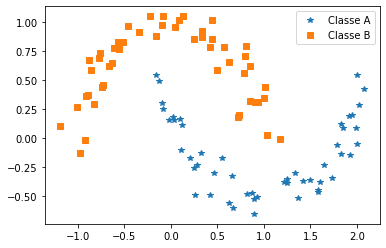
\includegraphics[width=0.41\textwidth]{moons.png}
        \end{figure}
        
        \begin{enumerate}
            \item Quais algoritmos de aprendizado de máquina, vistos no curso, poderiam ser utilizados para resolver este problema?
            \item Destes algoritmos, qual você escolheria? Discuta possíveis vantagens e desvantagens da sua escolha.
        \end{enumerate}

    \item Considere os seguintes métodos: regressão linear, regressão logística, árvores de decisão e redes neurais artificiais. Compare estes métodos em relação ao seu ''nível de inteligência``. 
        
    \item Para o que serve o algoritmo de backpropagation? Como ele influencia a escolha das funções de ativação e de custo (perda) de uma rede neural artificial?
    
    \item O que é overfitting? Quais são os indícios de que um modelo está sofrendo de overfitting? O que pode ser feito para reduzir overfitting em uma rede neural artificial?
    
    \pagebreak

    \item  Considere a rede neural abaixo:
    
    \begin{figure}[!ht]
        \centering
        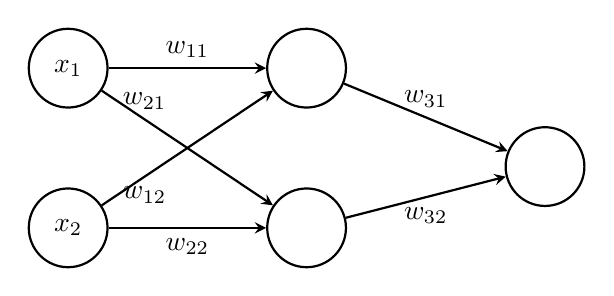
\begin{tikzpicture}[%
            neuron/.style={circle, draw, thick, minimum size=1cm},
            arrow/.style={->,>=stealth,thick}
        ]
        
        % Input neurons
        \node[neuron] (input1) at (0,0) {$x_1$};
        \node[neuron] (input2) [below=of input1] {$x_2$};
        
        % Hidden layer neurons
        \node[neuron] (hidden1) [right=2cm of input1] {};
        \node[neuron] (hidden2) [right=2cm of input2] {};
        
        % Output neuron
        \node[neuron] (output) [right=2cm of hidden1, yshift=-1.25cm] {};
        
        % Connect input layer to hidden layer
        \draw[arrow] (input1) -- (hidden1) node[midway, above] {$w_{11}$};
        \draw[arrow] (input1) -- (hidden2) node[near start, above] {$w_{21}$};
        \draw[arrow] (input2) -- (hidden1) node[near start, below] {$w_{12}$};
        \draw[arrow] (input2) -- (hidden2) node[midway, below] {$w_{22}$};
        
        % Connect hidden layer to output layer
        \draw[arrow] (hidden1) -- (output) node[midway, above] {$w_{31}$};
        \draw[arrow] (hidden2) -- (output) node[midway, below] {$w_{32}$};
        
        \end{tikzpicture}
    \end{figure}

    $w_{11}$ = $w_{21}$ = $w_{12}$ = $w_{22}$ = $w_{31}$ = $w_{32}$ = 1

    Esta rede tem como funções de ativação a função ReLU (Rectified Linear Unit) que pode ser definida como:

    \begin{equation}
        \text{ReLU}(x) = \max(0, x)
    \end{equation}

    A derivada da ReLU é definida como:

    \begin{equation}
            \frac{d}{dx}(\text{ReLU}(x)) =
            \begin{cases}
            1 & \text{if } x > 0 \\
            0 & \text{if } x \leq 0
            \end{cases}            
    \end{equation}


    \begin{enumerate}
        \item Calcule o gradiente do erro quadrado em relação à $w_{32}$ quando $\mathbf{x} = [2,1]$ e $y = 20$.
        \item Calcule o gradiente do erro quadrado em relação à $w_{22}$ quando $\mathbf{x} = [2,1]$ e $y = 20$. 
        \item Como $w_{32}$ e $w_{22}$ devem ser alterados de forma a diminuir o erro?   
    \end{enumerate}
    
    \item Considere a seguinte base de conhecimento (KB):
    \vspace{-0.5 cm}
    
    \begin{center}
        \begin{align*}
         a & \leftarrow b \wedge c. \\ 
         b & \leftarrow e. \\ 
         b & \leftarrow d. \\ 
         c &. \\ 
         d & \leftarrow h. \\ 
         e &. \\
         g & \leftarrow a \wedge b  \wedge e. \\
         f & \leftarrow a \wedge b. \\  
        \end{align*}
    \end{center}
    
    
    \begin{enumerate} 
        \item Apresente um modelo desta base de conhecimento.
        \item Apresente uma interpretação que não é um modelo desta base de conhecimento.
        \item Mostre um prova bottom-up para esta base de conhecimento. 
        \item Apresente uma prova top-down para a pergunta $ask$ $f$.
    \end{enumerate}
    
    \end{enumerate}

\end{document}

